\chapter{Background}
\section[]{Communicating Sequential Processes}
\section[]{Model Checking}
Model checking is the process of determining if a finite-state machine (FSM) is correct under a provided specification. It typically involves enumerating all possible states of an FSM and ensuring the correctness of each state. In software development, model checkers are beneficial in providing guarantees for safety-critical systems as well as concurrent systems. Concurrent systems can often cause issues with uncommon instruction execution interleavings that are not easily identifiable until long into a runtime. For example, deadlocks can occur when instructions being run by two processes are dependent on one another making progress. A simple example of a deadlock that can occur is the following interleaving of instructions executed by two processes, $\tau_1$ and $\tau_2$. 
\[
\begin{aligned}
& \tau_1: \text{ acquire lock A} \\
& \tau_2: \text{ acquire lock B} \\
& \tau_1: \text{ acquire lock B} \\
& \tau_2: \text{ acquire lock A}
\end{aligned}
\]
This simple interleaving results in $\tau_1$ blocking until it can acquire lock B, and $\tau_2$ blocking until it can acquire lock A, hence the program is in a deadlock. Due to the nature of concurrent systems, we could run our program and never experience this interleaving of instructions from occurring, hence we could deem our program deadlock-free. By instead abstracting our program as a model, and verifying the correctness using a model checker, we could exhaustively check all possible states (interleavings of concurrent processes) and catch this deadlock. 
\par
Alongside determining progress can be made within a system, model checkers are also used to guarantee the correctness of a specification. To demonstrate, we model a very simple 24-hour clock, where at each time step, we progress time by an hour.
\[
\begin{aligned}
& \tau_1: \text{time} \leftarrow \text{time} + 1
\end{aligned}
\]
Unlike the previous example, this process can always make progress so will not result in a deadlock, however, it is not a correct implementation of a 24-hour clock. We would like our 24-hour clock to only represent times in the range 1 to 24. By introducing a specification alongside our model, we can use a model checker to determine if all the states of our program adhere to the specification. In this instance, we would just need to specify a bound over our time variable.
\[
\{ \text{time} \mid \text{time} \in \mathbb{N}, 1 \leq \text{time} \leq 24 \}
\]
This is a simple example of a specification, that we can write in a specification language and use in tandem with our model to check the correctness of using a model checker.
\subsection[]{A Comparison Of Model Checkers}
Many model checkers have been invented for this reason, each with different focuses and specification languages. This section will comment on some of the more common model checkers and discuss their functionalities. \\
\subsubsection*{\textbf{PAT}}
Process Analysis Toolkit (PAT) is a self-contained framework to support composing, simulating and reasoning of concurrent, real-time systems \cite{pat}. PAT is based on Tony Hoare's CSP and extends the language using its library called CSP\#. CSP\# is a superset language of the original CSP, hence all classical CSP models can be verified with PAT. PAT has shown to be capable of verifying classical concurrent algorithms such as the dining philosophers problem. Alongside its verification capabilities, the PAT toolkit can be used to simulate real-world scenarios over specifications. 
\par
PAT's ability to determine the correctness of classical process algebra means it is a strong, widely applicable model checker.

\subsubsection*{\textbf{BLAST}}
BLAST is an automatic verification tool for checking the temporal safety properties of C programs. Given a C program and a temporal safety property, BLAST either statically proves the program satisfies the property or provides an execution path that exhibits a violation of the property \cite{blast}.
\par
Where BLAST is more interesting than PAT is that it no longer relies on process algebra. The model checker is capable of being run directly on a subset of C programs, no intermediate modelling is required. As an end-user tool, this is more generally applicable than PAT, there is no burden on developers to think about how to model their systems with process algebra and instead can directly get safety guarantees from their programs. BLAST handles the translation of C programs to an abstract reachability tree (ART), a labeled tree that represents a portion of the reachable state space of the program. Using a context-free reachability algorithm on this representation of a C program means temporal properties can be checked without the end programmer being required to think about what the control-flow automata for the program will look like.
\par
BLAST falls short when model-checking large C programs. More importantly, it is unable to provide any guarantees on concurrent programs. A strong driving factor in why developers choose to design systems in Elixir is its concurrent capabilities. 

\subsubsection*{\textbf{PRISM}}
PRISM is a probabilistic model checker, a tool for formal modelling and analysis of systems that exhibit random behavior or probabilistic behavior \cite{prism}. It has been used to analyse systems implementing random distributed algorithms.

\subsubsection*{\textbf{TLC}}
In 1980, Leslie Lamport discovered the Temporal Logic of Action (TLA) \cite{tla}. TLA is a logic system for specifying and reasoning about concurrent systems. Both the systems and their properties are represented in the same logic so that the assertion that a system meets its specification can be expressed by a logical implication.
\par
TLA is capable of specifying complex systems but in a typically verbose manner. Leslie Lamport introduced TLA+ \cite{tlaplus}, combining mathematical ideas with concepts from programming languages to create a specification language that would allow mathematicians to write specifications in 20 lines as opposed to 20 pages.
\begin{figure}[H]
    \begin{verbatim}
    ---------------------- MODULE HourClock ----------------------
    EXTENDS Naturals
    VARIABLE hr
    HCini == hr \in (1 .. 12)
    HCnxt == hr' = IF hr # 12 THEN hr + 1 ELSE 1
    HC == HCini /\ [][HCnxt]_hr
    --------------------------------------------------------------
    THEOREM HC => []HCini
    ==============================================================
    \end{verbatim}
    \caption{An example TLA+ Specification for an HourClock \cite{tlaplus}}
    \label{fig:hourclock_spec}
\end{figure}
\par
Furthering on from Leslie Lamport's discovery of these specification languages, Lamport created TLC \cite{tlc}, a model checker for the verification of TLA+ specifications. Similarly to BLAST, TLC builds a finite-state machine from the specification so the model checker can verify and debug invariance properties over it. TLC has been used to verify many large-scale, real-world systems specified in TLA+. Not only does it verify temporal properties of TLA+ specifications, but it can also model check PlusCal \cite{pluscal} algorithms. PlusCal is an algorithm language aimed to resemble that of pseudocode, but PlusCal algorithms can be automatically translated to TLA+ specifications to be reasoned about formally with TLC. We have already come across the concept of model-checking algorithms as opposed to specifications with BLAST, but instead of being strictly bound to the C programming language, PlusCal provides a more general framework agnostic of a choice of programming language allowing developers to separate reasoning about algorithms from their respective programs.

\subsubsection*{\textbf{SPIN}}
SPIN is an efficient verification system for models of distributed software systems. It has been used to detect design errors in applications ranging from high-level descriptions of distributed algorithms to detailed code \cite{spin}. Spin has a specification language, Process Meta Language (Promela), which the model checker uses to prove the correctness of asynchronous process interactions. Spin supports asynchronous process communication through channels, where processes can send and receive messages. Spin constructs labeled transition systems for respective processes from Promela specifications which it goes on to use for scheduling and to reason about properties of the model. Because many programming languages, such as GO \cite{go} rely on the creation of channels for asynchronous communication between processes, Promela becomes a natural solution to modelling these systems.
\begin{lstlisting}[caption={Example of a Promela specification that enqueues a message in a channel}]
mtype = { HELLO };
chan channel = [10] of { mtype };

init {
    channel ! HELLO;
}
\end{lstlisting}
\section[]{Elixir}
Elixir is a dynamic, functional language for building scalable and maintainable applications \cite{elixir}. Elixir programs run on the BEAM virtual machine\cite{beam}, which is also used to implement the Erlang programming language \cite{erlang}. Elixir was designed by José Valim and first released in 2012. Elixir is built on top of Erlang and hence inherits many of the abstractions designed for building distributed systems.
\par
BEAM is a virtual machine that executes user programs in the Erlang Runtime System (ERTS). BEAM is a register machine where all instructions operate on named registers containing Erlang terms such as integers or tuples.
\par
Elixir has begun to see use in industry, in particular in domains such as telecoms and instant messaging. The Phoenix Framework \cite{phoenix} is a framework for building interactive web applications natively in Elixir that can take advantage of Elixir's multi-processing and fault tolerance to build scalable web applications. The audio and video communication application Discord \cite{discord} uses Elixir to manage its 11 million concurrent users and the Financial Times \cite{ft} have begun migrating from Java to Elixir to enjoy the much smaller memory usage by comparison.
\par
Elixir supports multi-processing in two key ways: nodes and processes. Each node is an instance of BEAM (a single operating system process), when an Elixir program is executed, a new instance of BEAM is instantiated for it to run on. In contrast, an Elixir process is not an operating system process. An Elixir process is lightweight in terms of memory and CPU usage (even in comparison to threads that many other programming languages favour). Elixir processes can run concurrently with one another and are completely isolated from one another. Elixir processes communicate via message passing.
\begin{lstlisting}[language=Erlang, xleftmargin=.2\linewidth, caption={An example of spawn/1 and spawn/4 in Elixir for spawning a new lightweight process and a new Elixir node}]
    % Spawn a new process
    spawn(fn -> 1 + 2 end)

    % Create a new BEAM instance
    Node.spawn(:"node1@localhost", MyModule, :start, [])
\end{lstlisting}
\subsection[]{Shared Memory and Message Passing}
Two key concepts in inter-process communication (IPC) are shared memory models and message passing models. They are two techniques used to allow processes to send signals or share data between each other. In a shared memory model, a shared memory region is established in which multiple processes can read and write. Fig \ref{fig:shared_memory} shows a basic example of two processes that write to a shared in-memory array. Due to how often we see shared memory used in large-scale distributed systems, much work has been done in the verification of these systems using shared memory models. For example, Jon Mediero Iturrioz used Dafny \cite{dafny} to prove the correctness of concurrent programs that implement shared memory \cite{shared_memory_verification}. 
\begin{figure}[h]
    \centering
    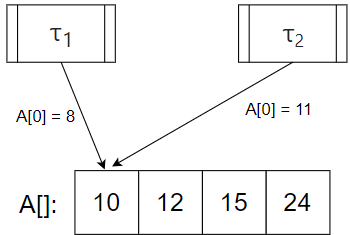
\includegraphics[width=0.4\textwidth]{images/shared_memory.png}
    \caption{An example of two processes writing to a shared in-memory array}
    \label{fig:shared_memory}
\end{figure}
\par
Elixir instead uses a message-passing model for IPC. More specifically, Elixir uses an actor-based model, where each process (actor) has its state and a message box to receive messages from other actors. Actors are responsible for sending a finite number of messages to other actors, spawning new actors and changing their behaviour based on the handling of messages received in the mailbox. Fig \ref{fig:actor_model} shows an example of how actors behave. The mailbox is not necessarily first in, first out (FIFO) but often implementations tend to be.
\begin{figure}[h]
    \centering
    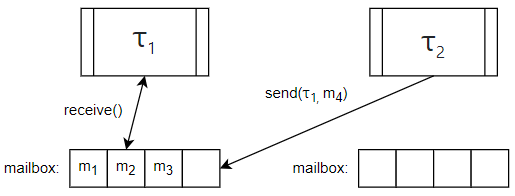
\includegraphics[width=0.6\textwidth]{images/actor_model.png}
    \caption{An example of actors sending and receiving messages under the actor model}
    \label{fig:actor_model}
\end{figure}
\par
In Elixir, a receive statement is used to read messages in the mailbox. The receive block looks through the mailbox for a message that matches a given pattern, if no messages match a given pattern, the process will block until one does.
\begin{lstlisting}[language=Erlang, xleftmargin=.2\linewidth, caption={An example of spawn/1 and spawn/4 in Elixir for spawning a new lightweight process and a new Elixir node}]
    % Example send in Elixir
    send self(), {:hello, "world"}

    % Example receive block in Elixir
    receive do
        {:hello, msg} -> IO.puts msg
    end
\end{lstlisting}
\subsection[]{Quote and Unquote}
\subsection[]{Metaprogramming}
\section[]{Existing Work}
\subsection[]{Lean}
\subsection[]{C Wolf}
\subsection[]{Dafny}
\subsection[]{Promela}
\subsection[]{Gomela}
\section[]{Modelling Elixir Programs in Promela}
\subsection[]{Basic Deadlock}
\subsection[]{Dining Philosophers}
\subsection[]{Preconditions and Postconditions}

